\section{Data Collection and Calibration}
\label{sec:data_calibration}

This section extends the project from the theoretical and numerical W3--W4 framework to the empirical components implemented in W5 and W6. The purpose of W5 is to collect and process market data for volatility analysis, while the purpose of W6 is to calibrate the Heston model to SPX implied-volatility information and the VIX futures term structure.

The earlier sections established the model, the Monte Carlo engine, and the CIR-based COS engine. The data and calibration stages connect these tools to market-facing tasks. In particular, W5 introduces realised and implied variance data, while W6 tests whether a one-factor Heston model can fit both SPX and VIX-related instruments simultaneously.

\subsection{W5 Data Collection and Exploratory Analysis}

The W5 component implements the empirical data pipeline used for volatility risk premium analysis and exploratory volatility-market diagnostics. The workflow includes downloading VIX daily index data, downloading SPX market data, obtaining VIX futures settlement data, computing realised variance from SPX returns, computing ex-post volatility risk premium, estimating ex-ante VRP using GARCH(1,1) forecasts, identifying crisis periods, and generating exploratory plots.

The main data inputs are:
\begin{itemize}
    \item VIX index levels;
    \item SPX index prices;
    \item VIX futures settlement data;
    \item a risk-free rate proxy.
\end{itemize}

The W5 pipeline covers the 2019--2024 period. This sample is useful because it contains both relatively calm volatility regimes and major stress episodes, including the 2020 COVID shock and the 2022 inflation shock. As a result, the dataset can be used not only for average behaviour, but also for crisis-regime interpretation.

\subsection{Realised Variance Estimation}

Realised variance is computed from SPX log returns. If \(S_i\) denotes the SPX level at observation time \(i\), the log return is
\begin{equation}
r_i
=
\log\left(
\frac{S_i}{S_{i-1}}
\right).
\end{equation}
The realised variance over a given period is computed as
\begin{equation}
RV_t
=
\sum_i r_i^2.
\end{equation}
Monthly realised variance is annualised where appropriate.

This realised-variance estimate is important because it provides the empirical counterpart to the theoretical integrated variance discussed in earlier sections. In the Monte Carlo part, realised variance was computed from simulated paths. In W5, the same concept is applied to market data using SPX returns.

\subsection{Implied Variance and Volatility Risk Premium}

The project approximates one-month implied variance from the VIX index:
\begin{equation}
IV_t
=
\frac{1}{12}
\left(
\frac{VIX_t}{100}
\right)^2.
\end{equation}
The one-month ex-post volatility risk premium is then computed as
\begin{equation}
VRP_t
=
IV_t
-
RV_{t,t+1M}.
\end{equation}
Equivalently,
\begin{equation}
VRP_t
=
\frac{1}{12}
\left(
\frac{VIX_t}{100}
\right)^2
-
RV_{t,t+1M}.
\end{equation}

A positive volatility risk premium means that implied variance is higher than subsequently realised variance. Economically, this is interpreted as compensation paid by investors who demand protection against future volatility. Sellers of volatility may earn this premium in normal periods, but they are exposed to large losses during market stress.

\subsection{W5 Empirical Findings}

The W5 exploratory analysis confirms several common stylised facts in volatility markets. First, the VIX index rises sharply during market stress. Second, implied variance is usually higher than future realised variance in calm market conditions. Third, the volatility risk premium is generally positive in normal regimes. Fourth, crisis periods can compress or reverse the premium. Finally, VIX and SPX returns are negatively related, especially during stress periods.

These findings are consistent with the interpretation of volatility as an insurance-like asset class. Market participants often pay a premium to protect against volatility spikes and equity drawdowns. This premium can be harvested in calm periods, but it carries crisis risk when realised variance rises sharply.

\subsection{W6 Joint SPX--VIX Calibration}

The W6 component implements a calibration framework for the Heston model. The goal is to test whether one set of Heston parameters can fit both the SPX implied-volatility surface and the VIX futures term structure.

The W6 workflow includes:
\begin{itemize}
    \item the Heston characteristic function for the log-stock process under the risk-neutral measure;
    \item a COS pricer for European SPX calls and puts;
    \item Black--Scholes implied-volatility inversion using Brent's method;
    \item SPX option-chain loading with CSV cache and synthetic SVI fallback;
    \item SPX calibration loss in vega-scaled price units;
    \item VIX futures calibration loss using the W4 COS engine;
    \item a joint SPX/VIX objective with a tunable mixing weight;
    \item a soft Feller-condition penalty;
    \item a two-stage optimiser combining differential evolution and L-BFGS-B.
\end{itemize}

The calibrated Heston parameter vector is
\begin{equation}
\Theta
=
(\kappa,\theta,\sigma_v,\rho,v_0).
\end{equation}
Here, \(\kappa\) controls mean-reversion speed, \(\theta\) is the long-run variance, \(\sigma_v\) is volatility of variance, \(\rho\) is stock-variance correlation, and \(v_0\) is initial variance.

\subsection{Calibration Objective}

Calibration means choosing model parameters so that model prices are close to market observations. A generic least-squares objective can be written as
\begin{equation}
\min_{\Theta}
\sum_{i=1}^{n}
w_i
\left(
P_i^{model}(\Theta)
-
P_i^{market}
\right)^2,
\end{equation}
where \(P_i^{market}\) is the observed market price or implied volatility, \(P_i^{model}(\Theta)\) is the corresponding model output, and \(w_i\) is a weight.

For SPX options, the model is evaluated through a Heston/COS option pricer and compared to the market implied-volatility surface. For VIX futures, the model-implied futures level is computed using the W4 VIX futures engine and compared to the observed futures curve.

The joint calibration objective combines SPX and VIX components:
\begin{equation}
\mathcal{L}_{joint}(\Theta)
=
\alpha \mathcal{L}_{SPX}(\Theta)
+
(1-\alpha)\mathcal{L}_{VIX}(\Theta)
+
\mathcal{P}_{Feller}(\Theta),
\end{equation}
where \(\alpha\in[0,1]\) controls the relative weight of the SPX and VIX markets, and \(\mathcal{P}_{Feller}\) is a soft penalty for violations of the Feller condition.

\subsection{Calibration Setup}

The calibration uses SPX option-chain information, VIX futures, and a flat risk-free rate proxy. The SPX maturity window is restricted to expirations between 14 and 365 days, and the moneyness range is restricted to log-moneyness within approximately \(\pm 0.4\). Only out-of-the-money calls and puts are used.

The Heston parameter bounds are:
\begin{center}
\begin{tabular}{lcc}
\toprule
Parameter & Lower bound & Upper bound \\
\midrule
\(\kappa\) & 0.10 & 15.00 \\
\(\theta\) & 0.005 & 0.250 \\
\(\sigma_v\) & 0.05 & 2.50 \\
\(\rho\) & -0.99 & 0.00 \\
\(v_0\) & 0.005 & 0.500 \\
\bottomrule
\end{tabular}
\end{center}

A soft quadratic penalty is applied when the Feller condition
\begin{equation}
2\kappa\theta \geq \sigma_v^2
\end{equation}
is violated. This does not strictly force the optimiser to remain inside the Feller region, but discourages parameter combinations that strongly violate the non-attainment condition for the zero boundary.

\subsection{Three Calibration Experiments}

W6 compares three calibration settings:
\begin{enumerate}
    \item SPX-only calibration;
    \item VIX-only calibration;
    \item joint SPX--VIX calibration.
\end{enumerate}

The calibrated parameter values are summarised in Table~\ref{tab:w6_calibrated_parameters}.

\begin{table}[htbp]
\centering
\begin{tabular}{lccccc}
\toprule
Calibration & \(\kappa\) & \(\theta\) & \(\sigma_v\) & \(\rho\) & \(v_0\) \\
\midrule
SPX-only & 0.966 & 0.064 & 0.352 & -0.937 & 0.033 \\
VIX-only & 0.209 & 0.250 & 0.050 & -0.700 & 0.005 \\
Joint \((\alpha=0.50)\) & 0.220 & 0.240 & 0.050 & -0.566 & 0.005 \\
\bottomrule
\end{tabular}
\caption{Calibrated Heston parameters under SPX-only, VIX-only, and joint calibration.}
\label{tab:w6_calibrated_parameters}
\end{table}

The calibration error comparison is shown in Table~\ref{tab:w6_calibration_errors}.

\begin{table}[htbp]
\centering
\begin{tabular}{lcc}
\toprule
Calibration & SPX IV RMSE & VIX futures RMSE \\
\midrule
SPX-only & 0.0159 & 5.90 \\
VIX-only & 0.0711 & 1.32 \\
Joint \((\alpha=0.50)\) & 0.0561 & 1.33 \\
\bottomrule
\end{tabular}
\caption{Calibration error comparison for SPX implied volatility and VIX futures.}
\label{tab:w6_calibration_errors}
\end{table}

\begin{figure}[htbp]
    \centering
    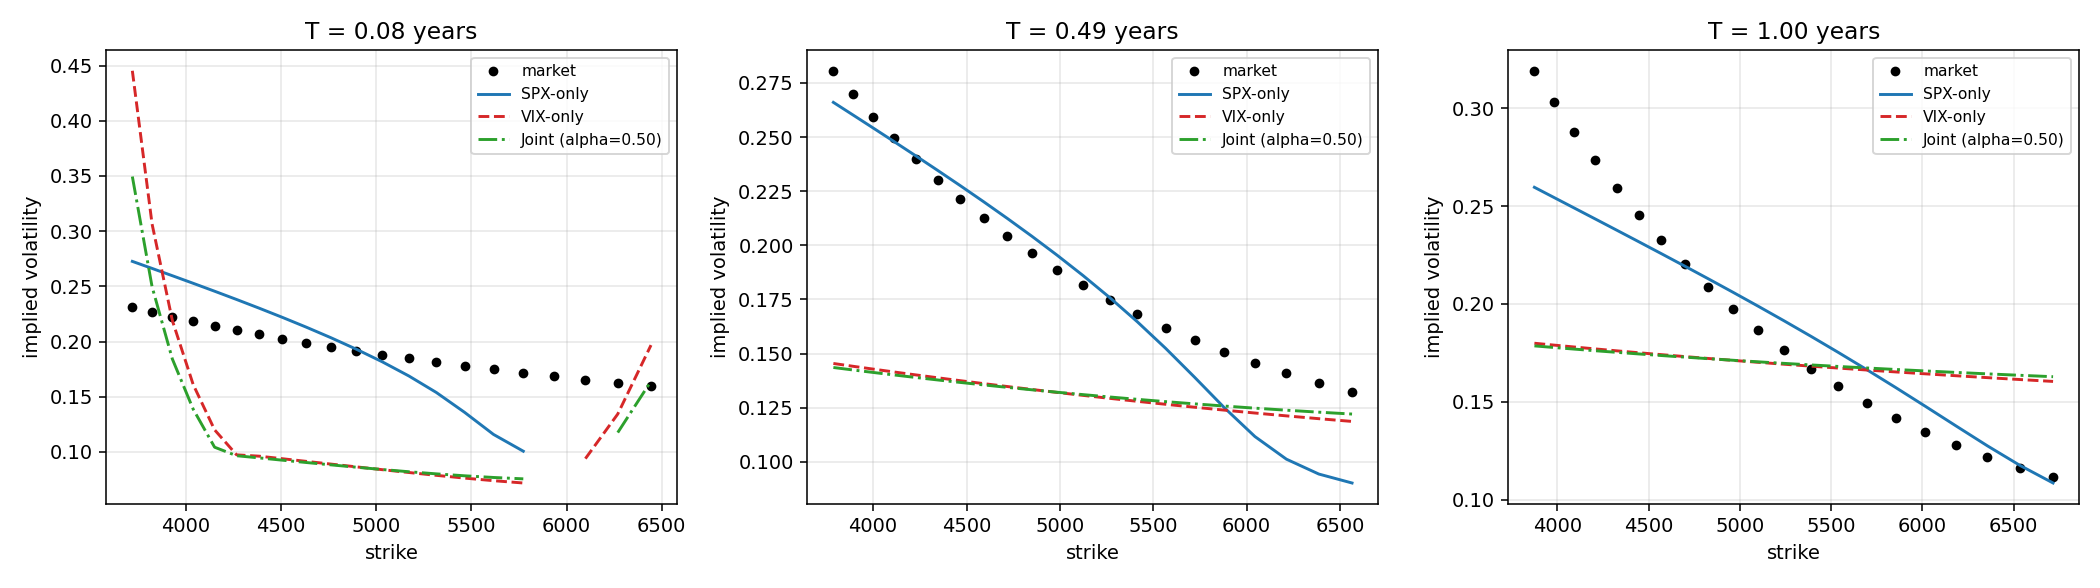
\includegraphics[width=0.88\textwidth]{figures/spx_smile_comparison.png}
    \caption{Comparison of SPX market and model-implied volatility smiles under different Heston calibration settings. The figure illustrates how SPX-only, VIX-only, and joint calibrations affect the fit to the SPX implied-volatility surface.}
    \label{fig:spx_smile_comparison}
\end{figure}

\begin{figure}[htbp]
    \centering
    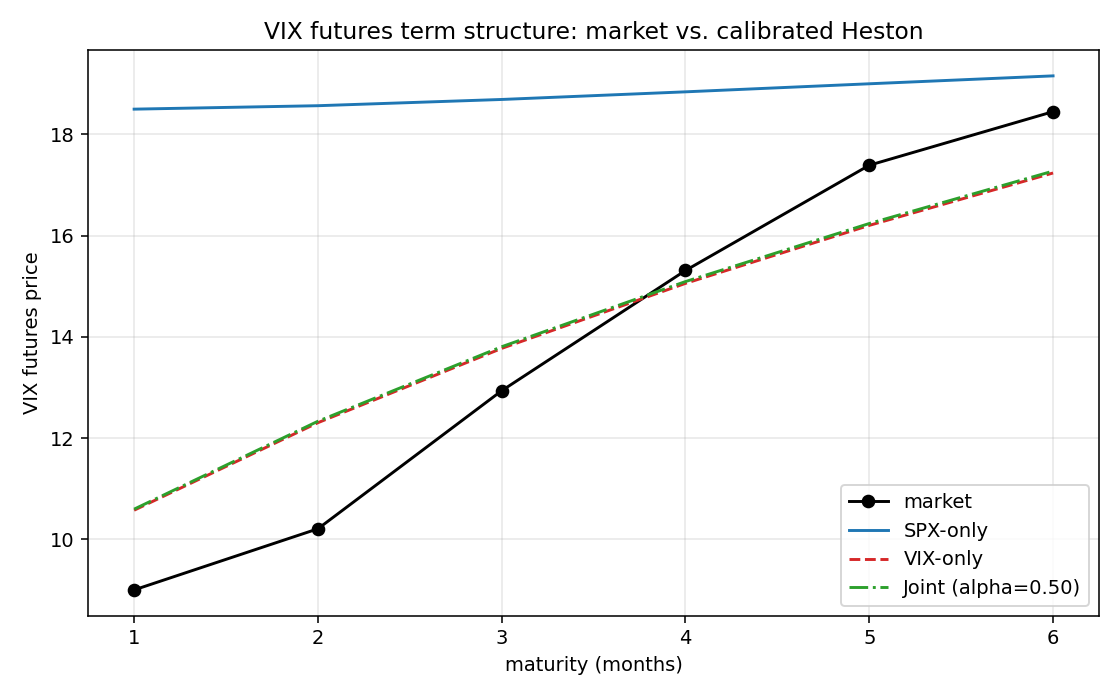
\includegraphics[width=0.88\textwidth]{figures/vix_futures_comparison.png}
    \caption{Comparison of market and model-implied VIX futures term structures under different calibration settings. The figure shows the difficulty of fitting VIX futures and SPX smiles simultaneously with a one-factor Heston model.}
    \label{fig:vix_futures_comparison}
\end{figure}

\begin{figure}[htbp]
    \centering
    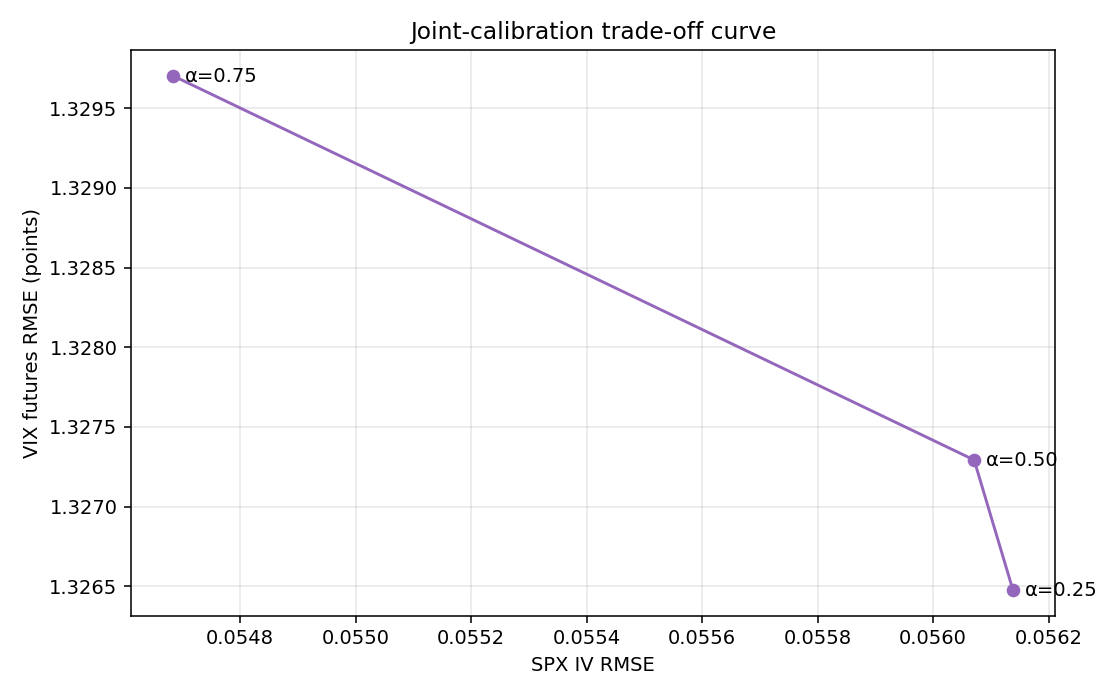
\includegraphics[width=0.82\textwidth]{figures/tradeoff_curve.png}
    \caption{Calibration trade-off between SPX implied-volatility RMSE and VIX futures RMSE. The figure visualises the structural limitation of the one-factor Heston model in joint SPX--VIX calibration.}
    \label{fig:tradeoff_curve}
\end{figure}

\subsection{Interpretation of Calibration Results}

The SPX-only calibration produces a strong fit to the SPX implied-volatility surface, with an SPX IV RMSE of \(0.0159\). However, the same parameter set produces a VIX futures RMSE of \(5.90\), indicating a poor fit to the VIX futures curve.

The VIX-only calibration produces a much better VIX futures RMSE of \(1.32\), but the SPX IV RMSE deteriorates to \(0.0711\). This means that the parameter set that fits the VIX futures curve does not reproduce the SPX volatility smile well.

The joint calibration with \(\alpha=0.50\) produces an SPX IV RMSE of \(0.0561\) and a VIX futures RMSE of \(1.33\). This result remains much closer to the VIX-only solution than to the SPX-only solution. The optimiser sacrifices SPX fit in order to keep the VIX futures curve close to the market.

Figures~\ref{fig:spx_smile_comparison}, \ref{fig:vix_futures_comparison}, and \ref{fig:tradeoff_curve} illustrate this trade-off visually. Together, they show that the one-factor Heston model can match one market dimension at a time, but struggles to fit the SPX smile and the VIX futures term structure simultaneously.

\subsection{Structural Implication}

The W6 calibration results support the central structural limitation discussed in the theory section: a one-factor Heston model can reproduce either the SPX smile or the VIX futures curve reasonably well, but not both simultaneously.

The SPX surface requires a strongly negative \(\rho\) and sufficient volatility-of-volatility to generate skew. The VIX futures curve is more directly controlled by the mean-reversion parameters and long-run variance level. Because a single variance factor must satisfy both markets at the same time, the model faces a structural trade-off.

This motivates the use of richer models in future work. Possible extensions include two-factor CIR models, forward-variance models, and rough-volatility models. These models introduce additional flexibility by decoupling short-term and long-term variance behaviour or by changing the regularity of the variance process.